\scanpage{12}
\mspage{\unsure{6}}
Program of the \deleted{paradigm \unsure{of the theory of|of the theory of}} \inserted{``gruppentheoretisches} Gleichnis'' (paradigm in terms of group theory) of \inserted{arithmetic :}\deleted{\unsure{arithmetic} absolute algebraic geometry (in characteristic 0).}

a) Give a complete ``gruppentheoretisch'' description of $\Gamma$

b) Give a complete description of all the elements of structure enumerated above, in important typical cases for $(\mathfrak X,D,J)$, some of which we indicate below.

\margin{We shall try to take $\mathfrak X$ proper as far as possible (even if it means completing\ldots)}

\uline{NB} When one has the elements of structure envisaged for $(\mathfrak X,D,J)$, one also has them automatically for \unsure{every|$\forall$} 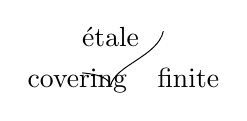
\begin{tikzpicture}[baseline=(rev012.base)]
\node[anchor=base west,inner sep=0pt] (rev012) at (0,0) {covering};
\node[anchor=base west,inner sep=0pt] at (1.65,0) {finite};
\node[anchor=base,inner sep=0pt] at (1.06,.52) {\inserted{étale}};
\draw[line width=.35pt] (.70,.19) .. controls (.91,.17) and (1.03,.13) .. (1.06,.03);
\draw[line width=.35pt] (1.06,.03) .. controls (1.12,.29) and (1.66,.40) .. (1.73,.72);
\end{tikzpicture} of $\mathfrak X'....$ One should make this point explicit with care, and also make explicit from the same viewpoints the ``hole-filling'' functors (by adding back 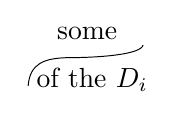
\begin{tikzpicture}[baseline=(des012.base)]
\node[anchor=base west,inner sep=0pt] (des012) at (.12,0) {of the $D_i$};
\node[anchor=base,inner sep=0pt] at (.77,.61) {\inserted{some}};
\draw[line width=.35pt] (.02,.02) .. controls (.04,.31) and (.23,.37) .. (.50,.38)
  .. controls (.93,.38) and (1.45,.42) .. (1.48,.54);
\end{tikzpicture} which one had removed) or ``hole-drilling'' 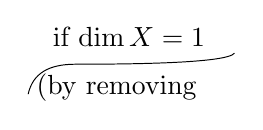
\begin{tikzpicture}[baseline=(en012.base)]
\node[anchor=base west,inner sep=0pt] (en012) at (.12,0) {(by removing};
\node[anchor=base,inner sep=0pt] at (1.30,.61) {\inserted{if $\dim\mathfrak X=1$}};
\draw[line width=.35pt] (.02,.01) .. controls (.08,.28) and (.29,.39) .. (.62,.39)
  .. controls (1.28,.39) and (2.54,.40) .. (2.64,.53);
\end{tikzpicture} some of the $\xi\in J$).
\mspage{11}
